% Options for packages loaded elsewhere
\PassOptionsToPackage{unicode}{hyperref}
\PassOptionsToPackage{hyphens}{url}
%
\documentclass[
  10pt,
  ignorenonframetext,
]{beamer}
\usepackage{pgfpages}
\setbeamertemplate{caption}[numbered]
\setbeamertemplate{caption label separator}{: }
\setbeamercolor{caption name}{fg=normal text.fg}
\beamertemplatenavigationsymbolsempty
% Prevent slide breaks in the middle of a paragraph
\widowpenalties 1 10000
\raggedbottom
\setbeamertemplate{part page}{
  \centering
  \begin{beamercolorbox}[sep=16pt,center]{part title}
    \usebeamerfont{part title}\insertpart\par
  \end{beamercolorbox}
}
\setbeamertemplate{section page}{
  \centering
  \begin{beamercolorbox}[sep=12pt,center]{part title}
    \usebeamerfont{section title}\insertsection\par
  \end{beamercolorbox}
}
\setbeamertemplate{subsection page}{
  \centering
  \begin{beamercolorbox}[sep=8pt,center]{part title}
    \usebeamerfont{subsection title}\insertsubsection\par
  \end{beamercolorbox}
}
\AtBeginPart{
  \frame{\partpage}
}
\AtBeginSection{
  \ifbibliography
  \else
    \frame{\sectionpage}
  \fi
}
\AtBeginSubsection{
  \frame{\subsectionpage}
}

\usepackage{amsmath,amssymb}
\usepackage{iftex}
\ifPDFTeX
  \usepackage[T1]{fontenc}
  \usepackage[utf8]{inputenc}
  \usepackage{textcomp} % provide euro and other symbols
\else % if luatex or xetex
  \usepackage{unicode-math}
  \defaultfontfeatures{Scale=MatchLowercase}
  \defaultfontfeatures[\rmfamily]{Ligatures=TeX,Scale=1}
\fi
\usetheme[block = fill, progressbar = frametitle]{metropolis}
\useinnertheme{circles}
\usepackage[]{AlegreyaSans}
\ifPDFTeX\else  
    % xetex/luatex font selection
\fi
% Use upquote if available, for straight quotes in verbatim environments
\IfFileExists{upquote.sty}{\usepackage{upquote}}{}
\IfFileExists{microtype.sty}{% use microtype if available
  \usepackage[]{microtype}
  \UseMicrotypeSet[protrusion]{basicmath} % disable protrusion for tt fonts
}{}
\makeatletter
\@ifundefined{KOMAClassName}{% if non-KOMA class
  \IfFileExists{parskip.sty}{%
    \usepackage{parskip}
  }{% else
    \setlength{\parindent}{0pt}
    \setlength{\parskip}{6pt plus 2pt minus 1pt}}
}{% if KOMA class
  \KOMAoptions{parskip=half}}
\makeatother
\usepackage{xcolor}
\newif\ifbibliography
\setlength{\emergencystretch}{3em} % prevent overfull lines
\setcounter{secnumdepth}{-\maxdimen} % remove section numbering


\providecommand{\tightlist}{%
  \setlength{\itemsep}{0pt}\setlength{\parskip}{0pt}}\usepackage{longtable,booktabs,array}
\usepackage{calc} % for calculating minipage widths
\usepackage{caption}
% Make caption package work with longtable
\makeatletter
\def\fnum@table{\tablename~\thetable}
\makeatother
\usepackage{graphicx}
\makeatletter
\def\maxwidth{\ifdim\Gin@nat@width>\linewidth\linewidth\else\Gin@nat@width\fi}
\def\maxheight{\ifdim\Gin@nat@height>\textheight\textheight\else\Gin@nat@height\fi}
\makeatother
% Scale images if necessary, so that they will not overflow the page
% margins by default, and it is still possible to overwrite the defaults
% using explicit options in \includegraphics[width, height, ...]{}
\setkeys{Gin}{width=\maxwidth,height=\maxheight,keepaspectratio}
% Set default figure placement to htbp
\makeatletter
\def\fps@figure{htbp}
\makeatother

\makeatletter
\makeatother
\makeatletter
\makeatother
\makeatletter
\@ifpackageloaded{caption}{}{\usepackage{caption}}
\AtBeginDocument{%
\ifdefined\contentsname
  \renewcommand*\contentsname{Table of contents}
\else
  \newcommand\contentsname{Table of contents}
\fi
\ifdefined\listfigurename
  \renewcommand*\listfigurename{List of Figures}
\else
  \newcommand\listfigurename{List of Figures}
\fi
\ifdefined\listtablename
  \renewcommand*\listtablename{List of Tables}
\else
  \newcommand\listtablename{List of Tables}
\fi
\ifdefined\figurename
  \renewcommand*\figurename{Figure}
\else
  \newcommand\figurename{Figure}
\fi
\ifdefined\tablename
  \renewcommand*\tablename{Table}
\else
  \newcommand\tablename{Table}
\fi
}
\@ifpackageloaded{float}{}{\usepackage{float}}
\floatstyle{ruled}
\@ifundefined{c@chapter}{\newfloat{codelisting}{h}{lop}}{\newfloat{codelisting}{h}{lop}[chapter]}
\floatname{codelisting}{Listing}
\newcommand*\listoflistings{\listof{codelisting}{List of Listings}}
\makeatother
\makeatletter
\@ifpackageloaded{caption}{}{\usepackage{caption}}
\@ifpackageloaded{subcaption}{}{\usepackage{subcaption}}
\makeatother
\makeatletter
\@ifpackageloaded{tcolorbox}{}{\usepackage[skins,breakable]{tcolorbox}}
\makeatother
\makeatletter
\@ifundefined{shadecolor}{\definecolor{shadecolor}{rgb}{.97, .97, .97}}
\makeatother
\makeatletter
\makeatother
\makeatletter
\makeatother
\ifLuaTeX
  \usepackage{selnolig}  % disable illegal ligatures
\fi
\IfFileExists{bookmark.sty}{\usepackage{bookmark}}{\usepackage{hyperref}}
\IfFileExists{xurl.sty}{\usepackage{xurl}}{} % add URL line breaks if available
\urlstyle{same} % disable monospaced font for URLs
\hypersetup{
  pdftitle={Shades of Blue},
  pdfauthor={Chaoyue R. Wang},
  hidelinks,
  pdfcreator={LaTeX via pandoc}}

\title{Shades of Blue}
\subtitle{Attitudinal Consequences of Racial Compositions of Police}
\author{Chaoyue R. Wang}
\date{April 6, 2023}
\institute{Independent Researcher}

\begin{document}
\frame{\titlepage}
\ifdefined\Shaded\renewenvironment{Shaded}{\begin{tcolorbox}[sharp corners, enhanced, frame hidden, interior hidden, breakable, boxrule=0pt, borderline west={3pt}{0pt}{shadecolor}]}{\end{tcolorbox}}\fi

\hypertarget{race-representation-and-policing}{%
\section{Race, Representation and
Policing}\label{race-representation-and-policing}}

\begin{frame}{Race and Policing in the U.S.}
\protect\hypertarget{race-and-policing-in-the-u.s.}{}
\begin{itemize}
\item
  \textbf{H1}: More representation of whites in local police workforce
  should lead to more favorable perceptions of police among white
  residents.
\item
  \textbf{H2}: When local police officers present a stronger white
  imagery, the occurrence of police violence will be less effective in
  persuading whites into more skeptical attitudes toward police.
\item
  \textbf{H2a}: The moderation effect of police's white imagery on white
  response to police violence will be strongest when the cases of such
  violence are racialized regarding their victims.
\end{itemize}
\end{frame}

\hypertarget{data-sources}{%
\section{Data Sources}\label{data-sources}}

\begin{frame}{Attitudes towards Policing}
\protect\hypertarget{attitudes-towards-policing}{}
\begin{figure}[tb]

{\centering 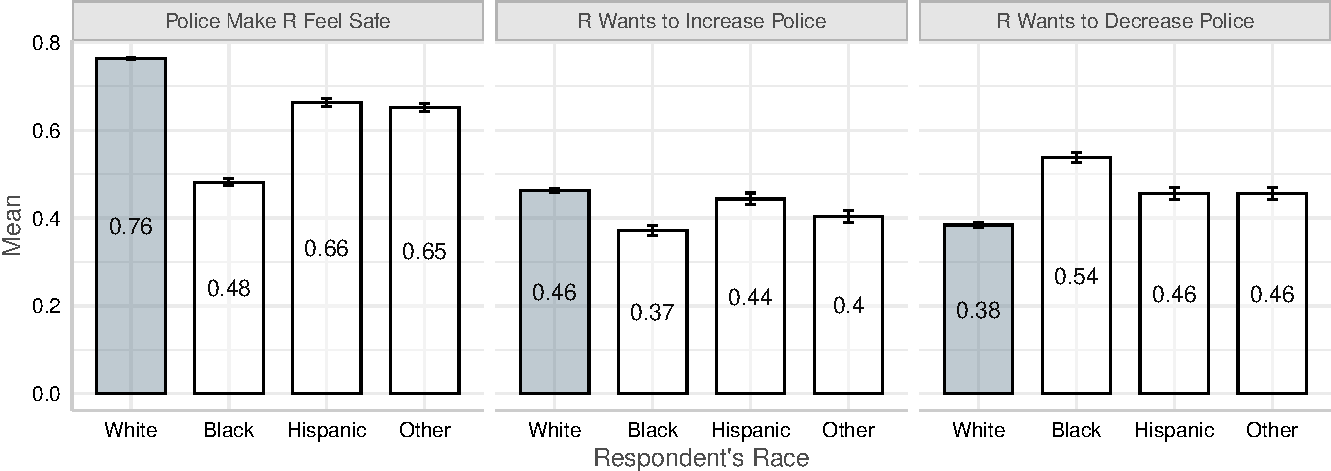
\includegraphics{slides_files/figure-beamer/fig-attitudes-1.pdf}

}

\caption{\label{fig-attitudes}\textbf{Attitudes toward Police by Race.}}

\end{figure}
\end{frame}

\begin{frame}{Racial Compositions of Police}
\protect\hypertarget{racial-compositions-of-police}{}
\begin{figure}

{\centering 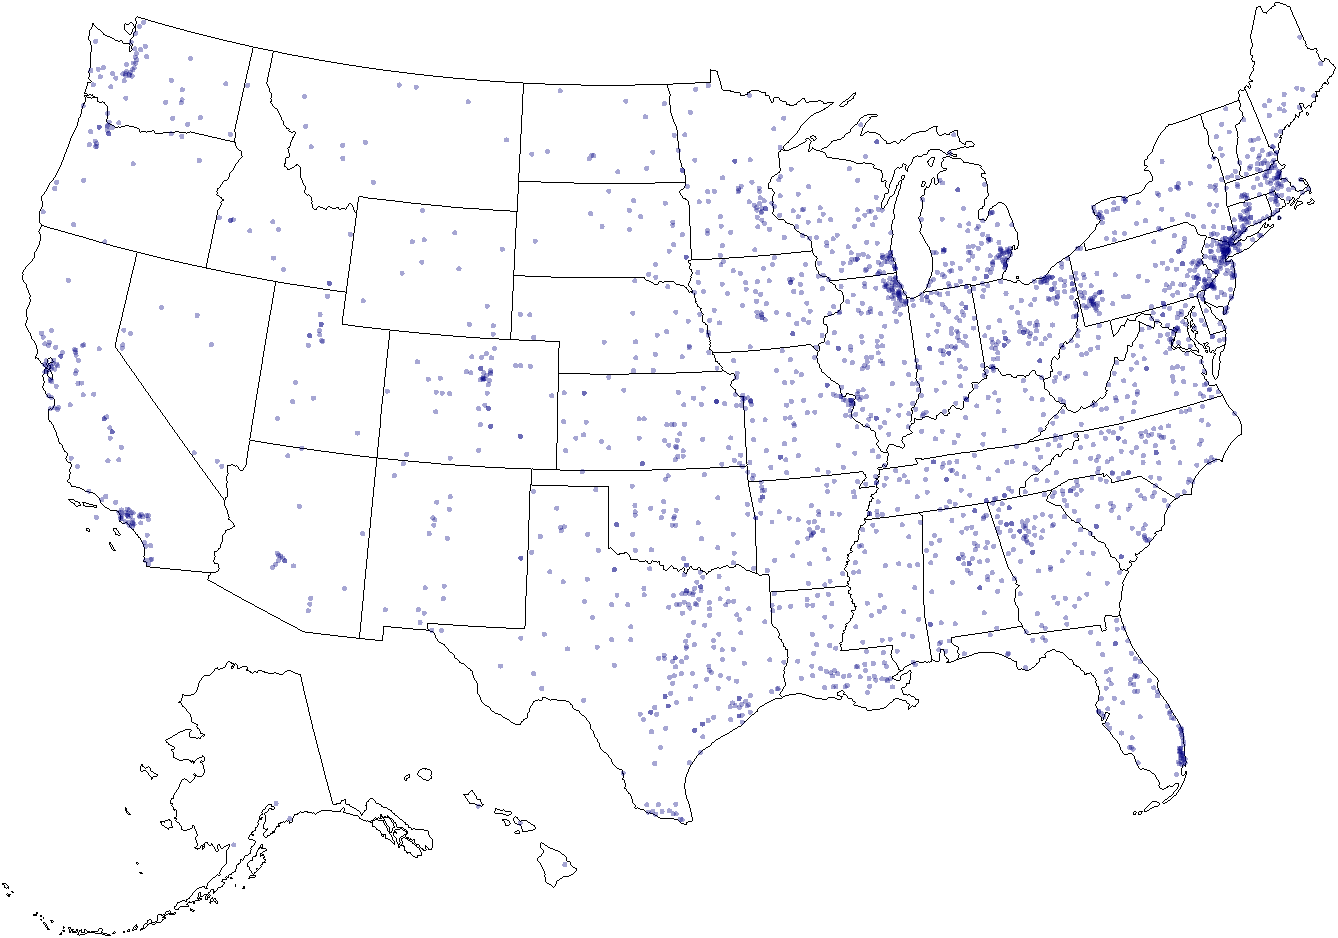
\includegraphics{slides_files/figure-beamer/fig-lemas-cover-1.pdf}

}

\caption{\label{fig-lemas-cover}\textbf{Geographic Coverage of 2016
LEMAS at the County Level.} Counties are colored blue where at least one
police department within its jurisdiction is surveyed in 2016 LEMAS.}

\end{figure}
\end{frame}

\begin{frame}{Police Brutality}
\protect\hypertarget{police-brutality}{}
\begin{itemize}
\item
  There have been no successful efforts by governmental agencies at
  either local or federal level to systematically document
  police-involved homicides.
\item
  Existing literature addressing police violence has usually turned to
  data voluntarily collected by advocacy groups, the most used of which
  is that of Mapping Police Violence project.
\item
  Drawing data points from other reliable sources of police-involved
  shootings and collecting its unique data through diverse channels
  including social media, local newspaper accounts, and police reports,
  the Mapping Police Violence project has by far the most detailed and
  accurate record of fatal shootings by police since 2013.
\end{itemize}
\end{frame}

\hypertarget{results}{%
\section{Results}\label{results}}

\begin{frame}{Attitudes towards Police and Policing}
\protect\hypertarget{attitudes-towards-police-and-policing}{}
\begin{figure}

{\centering 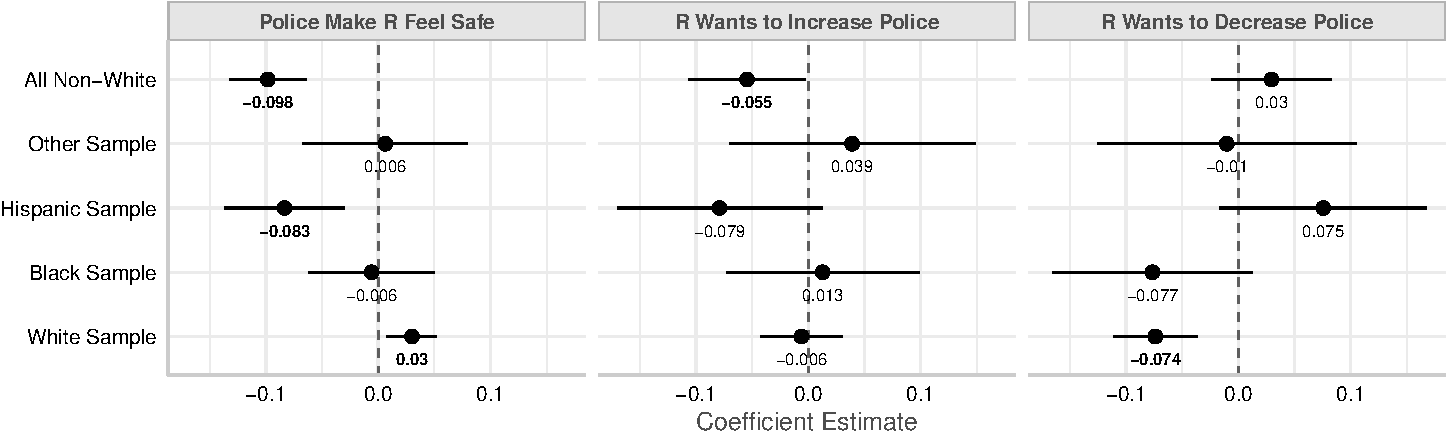
\includegraphics{slides_files/figure-beamer/fig-baseline-1.pdf}

}

\caption{\label{fig-baseline}\textbf{The Estiamted Relationship between
Racial Imagery of Local Police and White Attitudes on Policing.} Each
point indicates the coefficient estimate of the realted racial imagery
on policing attitudes out of an invididual regression among white
respondents in 2020 CES. 95\% confidence intervals are shown by the
range.}

\end{figure}
\end{frame}

\begin{frame}{Racial Divides on Policing}
\protect\hypertarget{racial-divides-on-policing}{}
\begin{table}

\end{table}
\end{frame}

\begin{frame}{Racial Divides on Policing}
\protect\hypertarget{racial-divides-on-policing-1}{}
\begin{figure}

{\centering 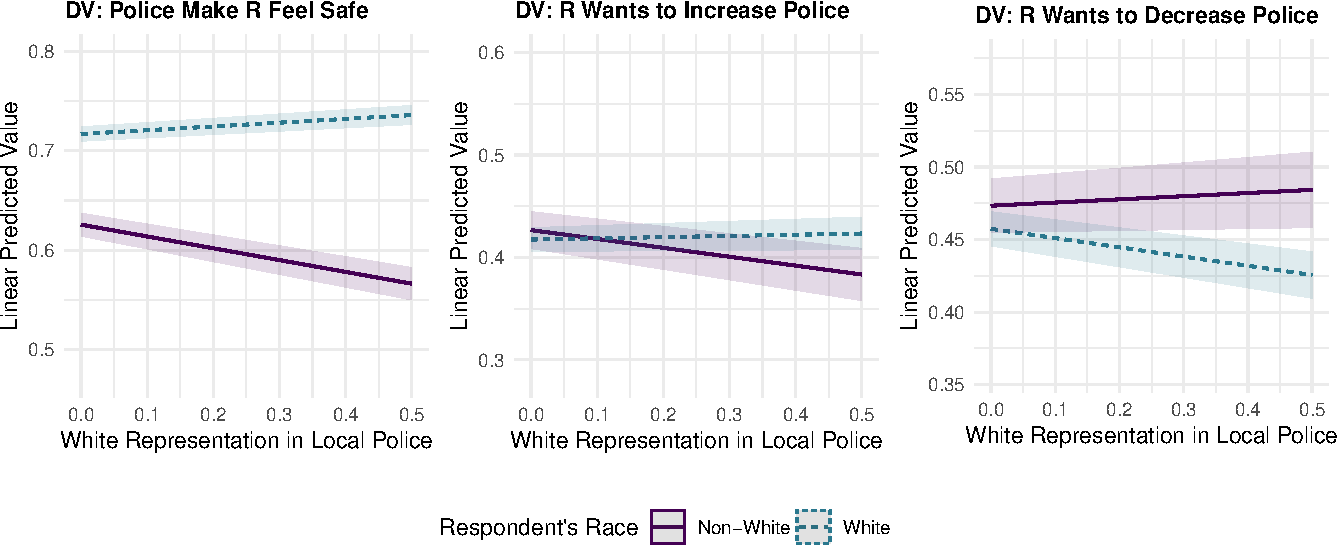
\includegraphics{slides_files/figure-beamer/fig-divides-1.pdf}

}

\caption{\label{fig-divides}\textbf{Racial Imagery of Local Police
Moderates Racial Divide regarding Attitudes on Policing.} Each plot
shows the racial divide on the outcome policing attitude as the white
imagery of local police increases. Ranges of racial imagery where racial
divide diminishes are colored red and indicated by blue reference lines.
The thicker black bar represents the observed range of white imagery of
police in our data.}

\end{figure}
\end{frame}

\begin{frame}{Reactions to Police Violence}
\protect\hypertarget{reactions-to-police-violence}{}
\begin{figure}

{\centering 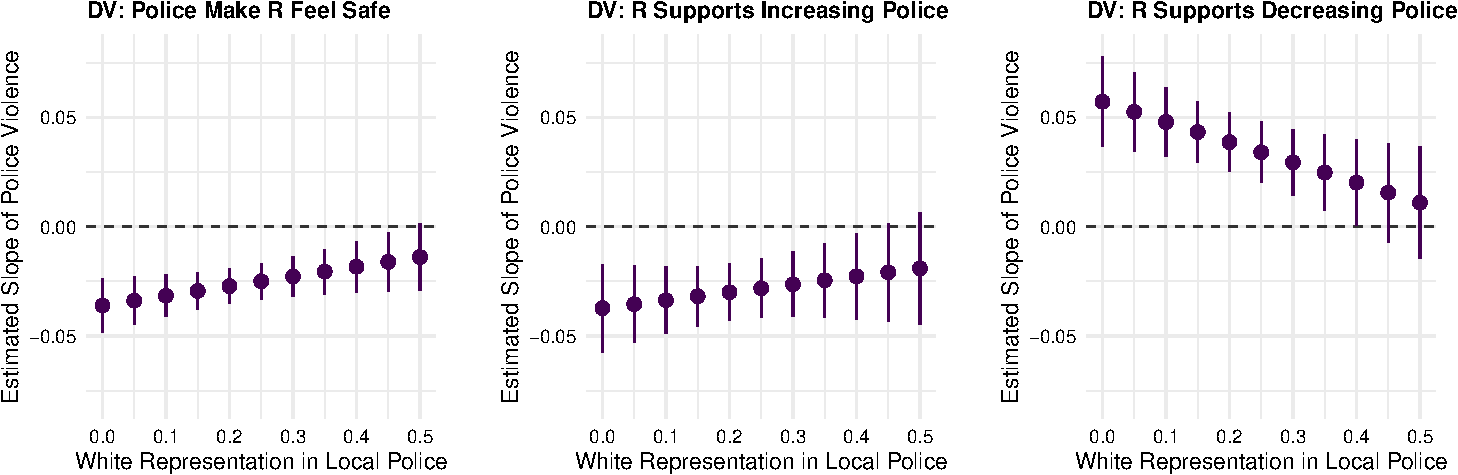
\includegraphics{slides_files/figure-beamer/fig-reaction-mod-1.pdf}

}

\caption{\label{fig-reaction-mod}\textbf{Racial Imagery of Local Police
Moderates Whites' Attitudinal Response to Police Violence.} At the each
level of racial imagery, whether there police violence happended in 2020
is indicated by the black-green scheme.}

\end{figure}
\end{frame}

\begin{frame}{Examine the Racial Dynamics}
\protect\hypertarget{examine-the-racial-dynamics}{}
\begin{figure}

{\centering 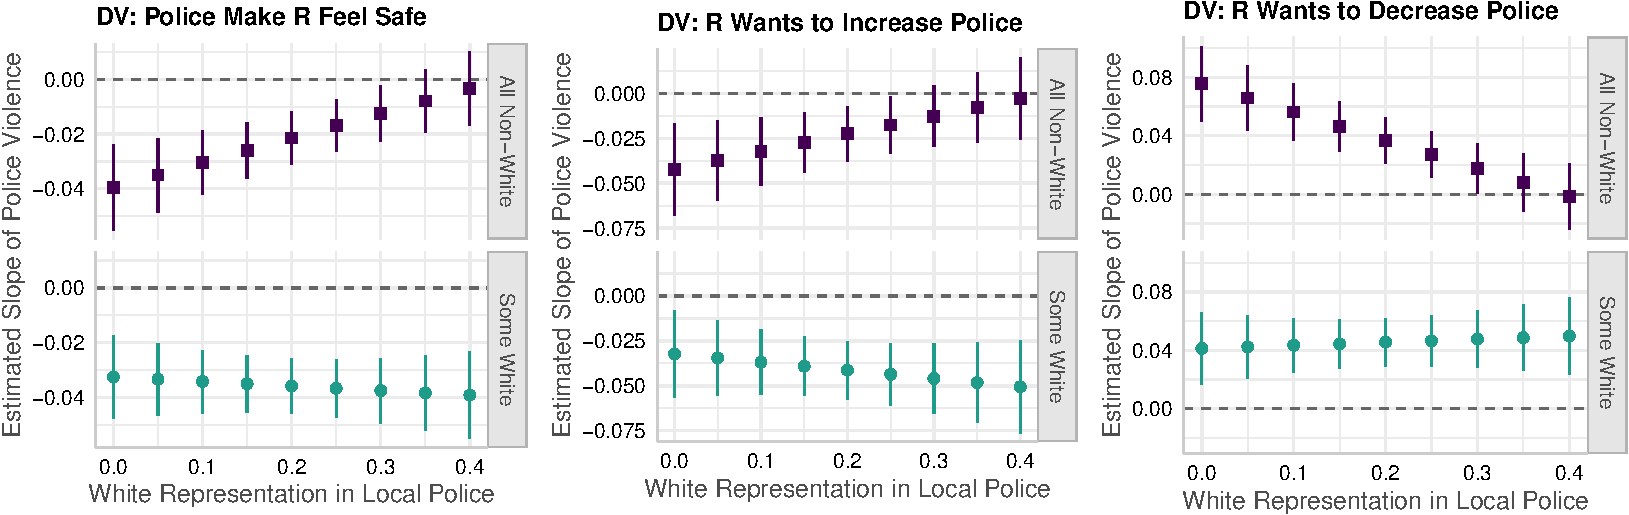
\includegraphics{slides_files/figure-beamer/fig-racial-component-1.pdf}

}

\caption{\label{fig-racial-component}\textbf{Moderating Effect of Racial
Imagery Depends upon Racial Groups Victimized by Police Violence.} At
the each level of racial imagery, the racial groups impacted by local
police violence in 2020 are indicated by the black-to-yellow scheme.}

\end{figure}
\end{frame}



\end{document}
